\setauthor{Moritz Eder}

Die Firma Macolution hat Kontakte zu Streaming- und Gesundheitsexperten. Diese Fachleute erstellen viele Videos, 
Übungen und Artikel zu diesen Themen. Der Auftraggeber will eine Applikation für diesen Kunden entwickeln, die folgende
Kriterien erfüllt:

\begin{itemize}
    \item User:innen müssen sich in der App nicht um die eigene Erstellung von Entspannungsmedien wie Texten oder Videos
    kümmern, weil diese Medien bereitgestellt werden, welche im Backend eingepflegt sind.
    \item Medien
    individuell favorisierbar und mehreren Kategorien zugeteilt sein, die per Suchleiste in der App einfach zu
    finden sind.
\end{itemize}

Das Minimum Viable Product (MVP) von Relaxoon soll realisiert werden, damit möglichst früh Feedback von Nutzer:innen
eingeholt werden kann, welches für die Weiterentwicklung und für die Verbesserung einer App essenziell ist.

Dies bestätigt der deutsche Content-Autor Philipp Steubel, der sich im amerikanischen Softwareunternehmen Asana
auf die Bereiche Marketing und 
Projektmanagement spezialisiert hat: "`Ein MVP ist sicherlich ein gutes Hilfsmittel, wenn es darum geht, den 
Entwicklungsprozess an den Kundenbedürfnissen zu orientieren. Immerhin bekommen Sie so schon während der 
Entwicklung des Produktes wertvolles Kundenfeedback. Somit erfahren Sie aber auch mehr über die Zielgruppe 
selbst, welche Personengruppen von dem Produkt bzw. dem Service überzeugt sind und wie Sie die Marketingkampagnen
aufsetzen können."' \cite{mvp}

% Personen, die oft gestresst vom Alltag sind, sollen durch Relaxoon wieder runterkommen
% und sich entspannen können, damit man sich wieder mit mehr Energie und einem klaren Kopf den
% nächsten Aufgaben stellen kann.

% Das Projekt soll zeigen, dass unter Verwendung des Open-Source headless CMS 'Strapi' und des mobilen
% React-Native Frontends eine App zur Wiedergabe von Mediendateien für verschiedene mobile Betriebssysteme
% und zur Stressbewältigung erstellt werden kann. 


% \begin{figure}[H]
%     \begin{minipage}{0.5\textwidth}
%         \centering
%         
\includegraphics[height=0.2\textwidth]{./pics/strapi-logo.png}
%         \caption{Logo Strapi}
%     \end{minipage}
%     \begin{minipage}{0.5\textwidth}
%         \centering
%         
\includegraphics[height=0.6\textwidth]{./pics/react-native-logo.png}
%         \caption{Logo React Native}
%     \end{minipage}
% \end{figure}

Wichtig dabei ist: 

\begin{itemize}
    \item die Feinabstimmung der Qualität der Inhalte
    \item die optimale Bereitstellung der sorgfältig ausgewählten Inhalte
    \item ein ansprechendes und benutzerfreundliches Design für den passenden ''Look and Feel'' der App.
\end{itemize}

\section{Use-Case-Diagramm (UCD)}

Für das Relaxoon gibt es im Wesentlichen zwei Hauptakteure: der/die Content-Manager:in und die Benutzer:innen der 
App. Diese Rollen interagieren mit verschiedenen Funktionen innerhalb der Anwendung, wie folgendermaßen 
dargestellt. Um die Übersichtlichkeit zu verbessern, wurde das UCD in zwei Teile aufgeteilt.

\begin{figure}[H]
    \centering
    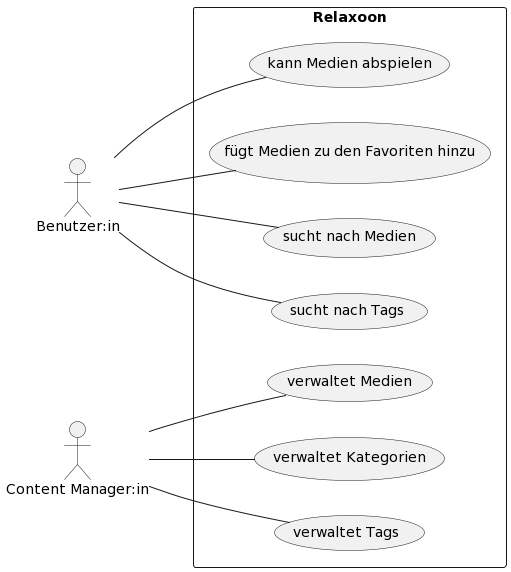
\includegraphics[height=\textwidth]{./pics/ucd1.png}
    \caption{Use-Case-Diagramm 1}
\end{figure}

% @startuml

% left to right direction
% skinparam packageStyle rectangle

% actor "Benutzer:in" as Benutzer
% actor "Content Manager:in" as ContentManager

%     package "Relaxoon" {
%         usecase "schaut Medien an" as UC1
%         usecase "favorisiert Medien" as UC2
%         usecase "sucht nach Medien" as UC3
%         usecase "sucht nach Tags" as UC31
%         usecase "erstellt neue Medien" as UC4
%         usecase "erstellt neue Kategorien" as UC5
%         usecase "erstellt neue Tags" as UC51
%         usecase "bearbeitet Medien" as UC6
%         usecase "bearbeitet Kategorien" as UC7
%         usecase "bearbeitet Tags" as UC71
%         usecase "ordnet Medien Kategorien zu" as UC8
%         usecase "ordnet Tags Medien zu" as UC81
%         usecase "löscht Medien" as UC9
%         usecase "löscht Kategorien" as UC10
%         usecase "löscht Tags" as UC11
%     }

%     Benutzer -- UC1
%     Benutzer -- UC2
%     Benutzer -- UC3
%     Benutzer -- UC31
%     ContentManager -- UC4
%     ContentManager -- UC5
%     ContentManager -- UC51
%     ContentManager -- UC6
%     ContentManager -- UC7
%     ContentManager -- UC71
%     ContentManager -- UC8
%     ContentManager -- UC81
%     ContentManager -- UC9
%     ContentManager -- UC10
%     ContentManager -- UC11

% @enduml

\textbf{Benutzer:in}
\begin{itemize}
    \item kann Medien abspielen: kann vorhandene Medien in der Anwendung anzeigen, um sie anzusehen oder zu konsumieren.
    \item fügt Medien zu den Favoriten hinzu: hat die Möglichkeit, bestimmte Medien als Favoriten zu markieren, um schnell auf sie zugreifen zu können.
    \item sucht nach Medien: kann in der Anwendung nach bestimmten Medien suchen, indem Suchkriterien eingegeben werden.
    \item sucht nach Tags: kann nach Medien suchen, indem nach bestimmten Tags oder Kategorien gefiltert wird, um gezielt Inhalte zu finden.
\end{itemize}
\textbf{Content Manager:in}
\begin{itemize}
    \item verwaltet Medien: kann Medien verwalten
    \item verwaltet Kategorien: kann Kategorien verwalten
    \item verwaltet Tags: kann Tags verwalten
\end{itemize}

\rule{\linewidth}{0.3pt}

Die Verwaltung der einzelnen Elemente wird im nächsten Diagramm genauer beschrieben.

\begin{figure}[H]
    \centering
    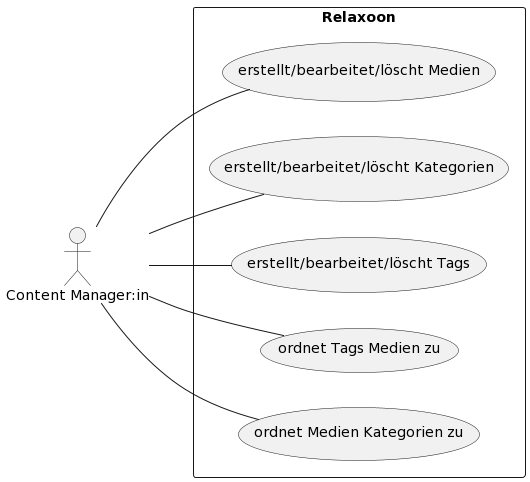
\includegraphics[height=0.84\textwidth]{./pics/ucd2.png}
    \caption{Use-Case-Diagramm 2}
\end{figure}

\newpage

\textbf{Content Manager:in}
\begin{itemize}
    \item erstellt/bearbeitet/löscht Medien: kann neue Medien in die Anwendung hochladen, vorhandene Medien bearbeiten und nicht mehr benötigte Medien entfernen.
    \item erstellt/bearbeitet/löscht Kategorien: kann neue Kategorien erstellen, bestehende Kategorien bearbeiten und überflüssige Kategorien löschen.
    \item erstellt/bearbeitet/löscht Tags: kann neue Tags erstellen, vorhandene Tags bearbeiten und ungenutzte Tags entfernen.
    \item ordnet Tags Medien zu: kann Tags bestimmten Medien zuweisen, um ihre Verschlagwortung und Klassifizierung zu optimieren.
    \item ordnet Medien Kategorien zu: kann Medien bestimmten Kategorien zuordnen, um ihre Einordnung und Auffindbarkeit in der Anwendung zu verbessern.
\end{itemize}
